\documentclass{article}
\usepackage{graphicx}
\usepackage{embedfile}

\embedfile[mimetype=application/pdf,desc=An icon for a PDF document]{openclipart-sixsixfive-matt-icons_application-x-pdf.pdf}
\embedfile[mimetype=image/jpeg,desc={This Hubble Space Telescope image shows a group of interacting galaxies called Arp 273. The larger of the spiral galaxies, known as UGC 1810, has a disk that is tidally distorted into a rose-like shape by the gravitational tidal pull of the companion galaxy below it, known as UGC 1813. A swath of blue jewels across the top is the combined light from clusters of intensely bright and hot young blue stars. These massive stars glow fiercely in ultraviolet light.}]{UGC_1810_and_UGC_1813_in_Arp_273_(captured_by_the_Hubble_Space_Telescope).jpg}

\begin{document}

\includegraphics[width=\linewidth,height=5cm,keepaspectratio]{openclipart-sixsixfive-matt-icons_application-x-pdf.pdf}
\clearpage
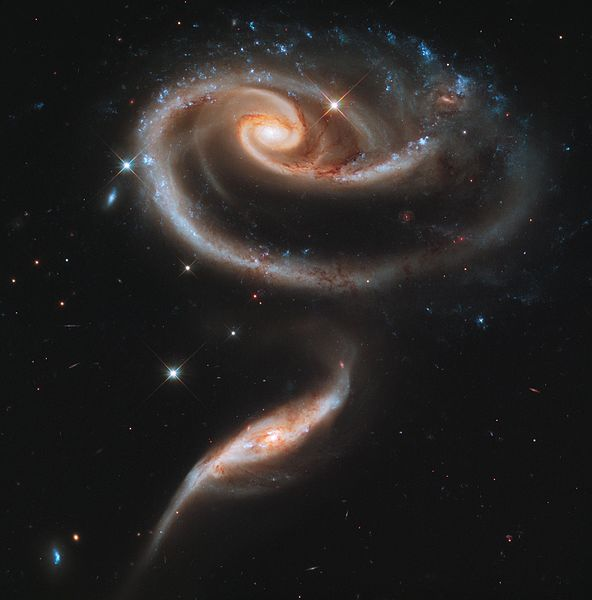
\includegraphics[width=\linewidth,height=5cm,keepaspectratio]{UGC_1810_and_UGC_1813_in_Arp_273_(captured_by_the_Hubble_Space_Telescope).jpg}
\end{document}
